\documentclass[12pt,twoside,singlespace]{mitthesis}
%\usepackage{lgrind}
%% These have been added at the request of the MIT Libraries, because
%% some PDF conversions mess up the ligatures.  -LB, 1/22/2014
\usepackage{tikz-feynman}
\usepackage{hyperref}
\usepackage{graphicx}
\usepackage{xspace}
\usepackage{xcolor}
\usepackage{cmap}
\usepackage[T1]{fontenc}
\usepackage{multirow}
\usepackage{textcomp}
\usepackage{siunitx}
\usepackage{rotating}
\pagestyle{plain}
\definecolor{violet}{RGB}{161,0,201}


\makeatletter
\def\hlinewd#1{%
	\noalign{\ifnum0=`} \fi \hrule \@height #1 \futurelet % 
   \reserved@a\@xhline}
\makeatother

%\newcommand{\Z}{\mbox{Z}}
%\newcommand{\W}{\mbox{W}}
\newcommand{\Z}{\ensuremath{\mathrm{Z}}}
\newcommand{\W}{\ensuremath{\mathrm{W}}}
%\newcommand{\met}{\ensuremath{\mspace{3mu}/\mspace{-12.0mu}E_{T}}}
%\newcommand{\metvector}{\ensuremath{\mspace{3mu}/\mspace{-12.0mu}\vec{E}_{T}}}
\newcommand{\mc}{Monte Carlo}
\newcommand{\MC}{\ensuremath{\textrm{MC}}\xspace}
\newcommand{\SM}{\mbox{SM}}
\newcommand{\lumiunc}{2.5\%}
%\newcommand{\lumi}{1.XXX\fbinv}%{1048~\pbinv}}
\newcommand{\invpb}{\ensuremath{\textrm{pb}^{\scriptscriptstyle -1}}}
\newcommand{\invfb}{\ensuremath{\textrm{fb}^{\scriptscriptstyle -1}}}
%\newcommand{\mev}{\ensuremath{\,\textrm{MeV}}}
%\newcommand{\gev}{\ensuremath{\,\textrm{GeV}}}
\newcommand{\tev}{\ensuremath{\,\textrm{TeV}}}
\newcommand{\Red}{\color{red}}
\newcommand{\Zmumu}{\ensuremath{Z\rightarrow \mu\mu}}
\newcommand{\Znunu}{\ensuremath{Z\rightarrow \nu\bar{\nu}}}
\newcommand{\Zboson}{\ensuremath{Z^0}}
\newcommand{\Zee}{\ensuremath{Z\rightarrow ee}}
\newcommand{\Zll}{\ensuremath{Z\rightarrow \ell\ell}\mbox{ with }\ensuremath{\ell=e,\mu}\xspace}
\newcommand{\rapidity}{\ensuremath{y}}
\newcommand{\pseudorapidity}{\ensuremath{\eta}}
\newcommand{\lepton}{\ensuremath{\ell}}
\newcommand{\TL}{{\bf Top-Left}}
\newcommand{\TR}{{\bf Top-Right}}
\newcommand{\BL}{{\bf Bottom-Left}}
\newcommand{\BR}{{\bf Bottom-Right}}
%\newcommand{\CL}{{\bf Center-Left}}
\newcommand{\CR}{{\bf Center-Right}}
\newcommand{\T}{{\bf Top}}
\newcommand{\B}{{\bf Bottom}}
\newcommand{\Right}{{\bf Right}}
\newcommand{\Left}{{\bf Left}}
\newcommand{\Center}{{\bf Center}}
\newcommand{\pythia}{{\tt \scshape pythia8}}
\newcommand{\geant}{{\tt \scshape geant}}
\newcommand{\madgraph}{\mbox{\tt \scshape MadGraph5}}
\newcommand{\powheg}{{\tt \scshape powheg}}
\newcommand{\sherpa}{{\tt \scshape sherpa}}
\newcommand{\herwigpp}{{\tt \scshape herwig++}}
\newcommand{\blackhat}{{\tt \scshape BlackHat}}
\newcommand{\amcatnlo}{\mbox{\tt \scshape MadGraph5\_aMC@NLO}}
\newcommand{\fewz}{\mbox{\tt FEWZ}}
\newcommand{\CMS}{{\tt CMS}\xspace}
\newcommand{\QCD}{{\tt QCD}\xspace}
\newcommand{\ptZ}{\ensuremath{p_T^{Z}}}
\newcommand{\ptG}{\ensuremath{p_T^{\gamma}}}
\newcommand{\phiso}{\ensuremath{PFIso_\textrm{photon}}}
\newcommand{\njets}{\ensuremath{n_\textrm{jets}}}
\newcommand{\phiStar}{\ensuremath{\phi^{\scriptscriptstyle *}_\eta}}
\newcommand{\RooUnfold}{{\scshape RooUnfold}}

%%% shortcut
\newcolumntype{d}[1]{D{.}{.}{#1}}

\newcommand{\tw}{\ensuremath{\mathrm{tW}}}
\newcommand{\dyee}{\ensuremath{Z/\gamma^*\to e^+e^-}}
\newcommand{\dymm}{\ensuremath{Z/\gamma^*\to\mu^+\mu^-}}
\newcommand{\dytt}{\ensuremath{Z/\gamma^*\to\tau^+\tau^-}}
\newcommand{\dyll}{\ensuremath{Z/\gamma^*\to\ell^+\ell^-}}
\newcommand{\WW}{\ensuremath{\W^+\W^-}}
\newcommand{\Lep}{\ensuremath{\ell}}
\newcommand{\mll}{\ensuremath{m_{\Lep\Lep}}}
\newcommand{\CLb}{\ensuremath{CL_\mathrm{b}}}

\newcommand{\nanob}{\mbox{{\rm ~nb}~}}
\newcommand{\fb}{\ensuremath{\mathrm{fb}}}
\newcommand{\pb}{\ensuremath{\mathrm{pb}}}
\newcommand{\ifb}{\ensuremath{\mathrm{fb^{-1}}}}
\newcommand{\ipb}{\ensuremath{\mathrm{pb^{-1}}}}
\newcommand{\grad}{\ensuremath{^{\circ}}}
%
% Special user made math symbols
%
\newcommand{\lsim}{\raisebox{-1.5mm}{$\:\stackrel{\textstyle{<}}{\textstyle{\sim}}\:$}}
\newcommand{\gsim}{\raisebox{-1.5mm}{$\:\stackrel{\textstyle{>}}{\textstyle{\sim}}\:$}}

% particles

\newcommand{\pipm}{\ensuremath{\pi^{\pm}}}
\newcommand{\pizero}{\ensuremath{\pi^{0}}}
\newcommand{\Hi}{\ensuremath{\mathrm{H}}}
\newcommand{\V}{\ensuremath{\mathrm{V}}}
\newcommand{\Wjets}{\ensuremath{\mathrm{W+jets}}}
\newcommand{\Zjets}{\ensuremath{\mathrm{Z+jets}}}
\newcommand{\Wt}{\ensuremath{\mathrm{Wt}}}
\newcommand{\Wstar}{\ensuremath{\mathrm{W}^{*}}}
\newcommand{\Wparenthesisstar}{\ensuremath{\mathrm{W}^{(*)}}}
\newcommand{\Zstar}{\ensuremath{\mathrm{Z}^{*}}}
%\newcommand{\Wpm}{\ensuremath{\W^{\pm}}}
\newcommand{\ZZ}{\ensuremath{\Z\Z}}
\newcommand{\WZ}{\ensuremath{\W\Z}}
\newcommand{\El}{\ensuremath{\mathrm{e}}}
\newcommand{\Elp}{\ensuremath{\mathrm{e}^{+}}}
\newcommand{\Elm}{\ensuremath{\mathrm{e}^{-}}}
\newcommand{\Elpm}{\ensuremath{\mathrm{e}^{\pm}}}
\newcommand{\Elmp}{\ensuremath{\mathrm{e}^{\mp}}}
\newcommand{\M}{\ensuremath{\mu}}
\newcommand{\Mp}{\ensuremath{\mu^{+}}}
\newcommand{\Mm}{\ensuremath{\mu^{-}}}
\newcommand{\Mpm}{\ensuremath{\mu^{\pm}}}
\newcommand{\Mmp}{\ensuremath{\mu^{\mp}}}
\newcommand{\Tau}{\ensuremath{\tau}}
\newcommand{\Nu}{\ensuremath{\nu}}
\newcommand{\Nubar}{\ensuremath{\bar{\nu}}}
\newcommand{\Lepp}{\ensuremath{\ell^{+}}}
\newcommand{\Lepm}{\ensuremath{\ell^{-}}}
\newcommand{\Lprime}{\ensuremath{\Lep^{\prime}}}
\newcommand{\Prot}{\ensuremath{\mathrm{p}}}
\newcommand{\Pbar}{\ensuremath{\bar{\mathrm{p}}}}
\newcommand{\PP}{\Prot\Prot}
\newcommand{\PPbar}{\Prot\Pbar}
\newcommand{\qq}{\ensuremath{\mathrm{q}\mathrm{q}}}
%\newcommand{\bbbar}{\ensuremath{\mathrm{b}\bar{\mathrm{b}}}}
\newcommand{\Wtb}{\ensuremath{\W\mathrm{t}\mathrm{b}}}
\newcommand{\Top}{\ensuremath{\mathrm{t}}}
\newcommand{\Bot}{\ensuremath{\mathrm{b}}}
\newcommand{\Atop}{\ensuremath{\bar{\mathrm{t}}}}
\newcommand{\Abot}{\ensuremath{\bar{\mathrm{b}}}}
\newcommand{\WH}{\ensuremath{\W\Hi}}
\newcommand{\ZH}{\ensuremath{\Z\Hi}}
% arrow
\newcommand{\To}{\ensuremath{\rightarrow}}

% masses
\newcommand{\mHi}{\ensuremath{m_{\mathrm{H}}}}
\newcommand{\mW}{\ensuremath{m_{\mathrm{W}}}}
\newcommand{\mZ}{\ensuremath{m_{\mathrm{Z}}}}
\newcommand{\mt}{\ensuremath{m_{T}}}

% kinematics
\newcommand{\ptveto}{\ensuremath{\pt^\mathrm{veto}}}
\newcommand{\ptl}{\ensuremath{p_\perp^{\Lep}}}
\newcommand{\ptlmax}{\ensuremath{p_{\mathrm{T}}^{\Lep,\mathrm{max}}}}
\newcommand{\ptlmin}{\ensuremath{p_{\mathrm{T}}^{\Lep,\mathrm{min}}}}
\newcommand{\Et}{\ensuremath{E_\mathrm{T}}}
\newcommand{\met}{\ensuremath{\Et^{\mathrm{miss}}}}
\newcommand{\delphill}{\ensuremath{\Delta\phi_{\Lep\Lep}}}
\newcommand{\deletall}{\ensuremath{\Delta\eta_{\Lep\Lep}}}
\newcommand{\delphimetl}{\ensuremath{\Delta\phi_{\met\Lep}}}
\newcommand{\delR}{\ensuremath{\Delta R}}
\newcommand{\Eta}{\ensuremath{\eta}}
\newcommand{\mT}{\ensuremath{m_{\mathrm{T}}^{\ell\ell\met}}}
\newcommand{\vmet}{\ensuremath{\vec{E}_\mathrm{T}}^{\text{miss}}}
\newcommand{\vg}{\ensuremath{\vec{\gamma}_\mathrm{T}}}
\newcommand{\delphillmetg}{\ensuremath{\Delta\phi(\Lep\Lep,\vmet+\vg})}

\newcommand{\pfmet}{\ensuremath{E_\mathrm{T,PF}^{\mathrm{miss}}}}
%efficiencies
\newcommand{\effsig}{\ensuremath{\varepsilon_{\mathrm{bkg}}^{\mathrm{S}}}}
\newcommand{\effnorm}{\ensuremath{\varepsilon_{\mathrm{bkg}}^{\mathrm{N}}}}
\newcommand{\Nsig}{\ensuremath{N_{\mathrm{bkg}}^{\mathrm{S}}}}
\newcommand{\Nnorm}{\ensuremath{N_{\mathrm{bkg}}^{\mathrm{N}}}}

% processes
\newcommand{\zee}{\ensuremath{Z\to e^+e^-}}
\newcommand{\zmm}{\ensuremath{Z\to\mu^+\mu^-}}
\newcommand{\ztt}{\ensuremath{Z\to\tau^+\tau^-}}
\newcommand{\zll}{\ensuremath{Z\to\ell^+\ell^-}}
%\newcommand{\ttbar}{\ensuremath{t\bar{t}}}
\newcommand{\ppww}{\ensuremath{pp \to W^+W^-}}
\newcommand{\wwll}{\ensuremath{WW\to \ell^+\ell^-}}
\newcommand{\wwlnln}{\ensuremath{W^+W^-\to \ell^+\nu \ell^-\bar{\nu}}}
\newcommand{\hww}{\ensuremath{\Hi \to \WW}}
\newcommand{\wz}{\ensuremath{WZ}}
\newcommand{\zz}{\ensuremath{ZZ}}
\newcommand{\wgamma}{\ensuremath{W\gamma}}
\newcommand{\wjets}{\ensuremath{W+}jets}
\newcommand{\singletopt}{\ensuremath{t} ($t$-chan)}
\newcommand{\singletops}{\ensuremath{t} ($s$-chan)}

%other
\def\fixme{({\bf \color{red}FIXME})}
\newcommand{\ee}{\ensuremath{ee}}
\newcommand{\emu}{\ensuremath{e\mu}}

% integrated luminosity
\newcommand{\usedLumiWithSyst}{35.9~\pm~0.9~\ifb}
\newcommand{\usedLumi}{35.9~\ifb}

\input{pennames.sty}
\input{ptdr-definitions.sty}
\begin{document}

\begin{figure} % ZZ
 \centering
 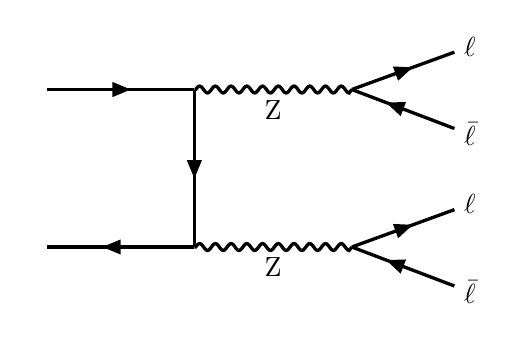
\begin{tikzpicture} % ZZ to 4l LO
  \begin{feynman}
   \vertex (q1) {\(\boldsymbol{\Pq}\)};
   \vertex [below= 2cm of q1] (q2) {\(\boldsymbol{\Paq}\)};
   \vertex [right= 2cm of q1] (a);
   \vertex [right= 2cm of q2] (b);
   \vertex [right= 2cm of a] (c);
   \vertex [right= 2cm of b] (d);
   \vertex [right= 1.5cm of c] (e);
   \vertex [right= 1.5cm of d] (f);
   \vertex [above= 0.3cm of e] (f1) {\(\boldsymbol{\ell}\)};
   \vertex [below= 0.3cm of e] (f2) {\(\boldsymbol{\bar{\ell}}\)};
   \vertex [above= 0.3cm of f] (f3) {\(\boldsymbol{\ell}\)};
   \vertex [below= 0.3cm of f] (f4) {\(\boldsymbol{\bar{\ell}}\)};
   
   \diagram* {
    (q1) -- [fermion, very thick] (a),
    (q2) -- [anti fermion, very thick] (b),
    (a) -- [fermion, very thick] (b),
    (a) -- [boson, very thick, edge label'=\(\boldsymbol{\Z}\)] (c),
    (b) -- [boson, very thick, edge label'=\(\boldsymbol{\Z}\)] (d),
    (c) -- [fermion, very thick] (f1),
    (c) -- [anti fermion, very thick] (f2),
    (d) -- [fermion, very thick] (f3),
    (d) -- [anti fermion, very thick] (f4),
   };
  \end{feynman}
 \end{tikzpicture} \hspace{1cm}
 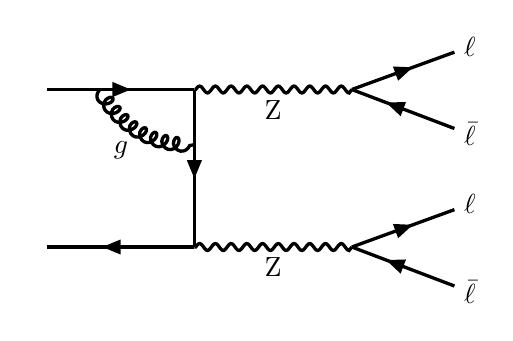
\begin{tikzpicture} %% ZZ to 4l NLO QCD
  \begin{feynman}
   \vertex (q1) {\(\boldsymbol{\Pq}\)};
   \vertex [below= 2cm of q1] (q2) {\(\boldsymbol{\Paq}\)};
   \vertex [right= 2cm of q1] (a);
   \vertex [right= 2cm of q2] (b);
   \vertex [right= 2cm of a] (c);
   \vertex [right= 2cm of b] (d);
   \vertex [right= 1.5cm of c] (e);
   \vertex [right= 1.5cm of d] (f);
   \vertex [above= 0.3cm of e] (f1) {\(\boldsymbol{\ell}\)};
   \vertex [below= 0.3cm of e] (f2) {\(\boldsymbol{\bar{\ell}}\)};
   \vertex [above= 0.3cm of f] (f3) {\(\boldsymbol{\ell}\)};
   \vertex [below= 0.3cm of f] (f4) {\(\boldsymbol{\bar{\ell}}\)};
   \vertex [right= 0.8cm of q1] (g1);
   \vertex [below= 0.7cm of a] (g2);
   
   \diagram* {
    (q1) -- [fermion, very thick] (a),
    (q2) -- [anti fermion, very thick] (b),
    (a) -- [fermion, very thick] (b),
    (a) -- [boson, very thick, edge label'=\(\boldsymbol{\Z}\)] (c),
    (b) -- [boson, very thick, edge label'=\(\boldsymbol{\Z}\)] (d),
    (c) -- [fermion, very thick] (f1),
    (c) -- [anti fermion, very thick] (f2),
    (d) -- [fermion, very thick] (f3),
    (d) -- [anti fermion, very thick] (f4),
    (g1) -- [gluon, very thick, bend right, edge label'=\(\boldsymbol{g}\)] (g2),
   };
  \end{feynman}
 \end{tikzpicture}  \vspace{1cm}
 
 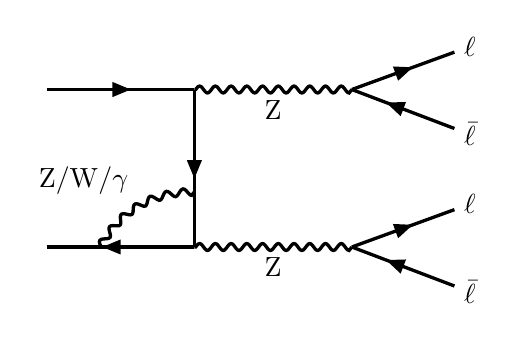
\begin{tikzpicture} %% ZZ to 4l NLO only EW
  \begin{feynman}
   \vertex (q1) {\(\boldsymbol{\Pq}\)};
   \vertex [below= 2cm of q1] (q2) {\(\boldsymbol{\Paq}\)};
   \vertex [right= 2cm of q1] (a);
   \vertex [right= 2cm of q2] (b);
   \vertex [right= 2cm of a] (c);
   \vertex [right= 2cm of b] (d);
   \vertex [right= 1.5cm of c] (e);
   \vertex [right= 1.5cm of d] (f);
   \vertex [above= 0.3cm of e] (f1) {\(\boldsymbol{\ell}\)};
   \vertex [below= 0.3cm of e] (f2) {\(\boldsymbol{\bar{\ell}}\)};
   \vertex [above= 0.3cm of f] (f3) {\(\boldsymbol{\ell}\)};
   \vertex [below= 0.3cm of f] (f4) {\(\boldsymbol{\bar{\ell}}\)};
   \vertex [right= 0.8cm of q2] (V1);
   \vertex [above= 0.7cm of b] (V2);
   
   \diagram* {
    (q1) -- [fermion, very thick] (a),
    (q2) -- [anti fermion, very thick] (b),
    (a) -- [fermion, very thick] (b),
    (a) -- [boson, very thick, edge label'=\(\boldsymbol{\Z}\)] (c),
    (b) -- [boson, very thick, edge label'=\(\boldsymbol{\Z}\)] (d),
    (c) -- [fermion, very thick] (f1),
    (c) -- [anti fermion, very thick] (f2),
    (d) -- [fermion, very thick] (f3),
    (d) -- [anti fermion, very thick] (f4),
    (V1) -- [boson, very thick, bend left, edge label=\(\boldsymbol{\Z/\W/\gamma}\)] (V2),
   };
  \end{feynman}
 \end{tikzpicture} \hspace{1cm}
 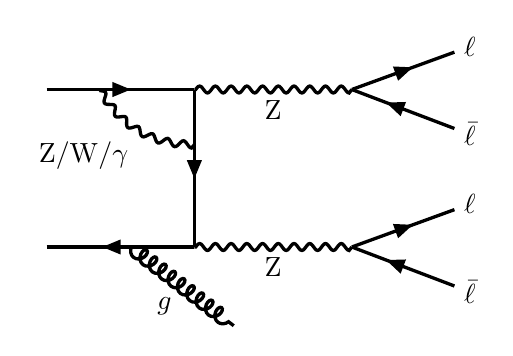
\begin{tikzpicture} %% ZZ to 4l NLO EW and QCD
  \begin{feynman}
   \vertex (q1) {\(\boldsymbol{\Pq}\)};
   \vertex [below= 2cm of q1] (q2) {\(\boldsymbol{\Paq}\)};
   \vertex [right= 2cm of q1] (a);
   \vertex [right= 2cm of q2] (b);
   \vertex [right= 2cm of a] (c);
   \vertex [right= 2cm of b] (d);
   \vertex [right= 1.5cm of c] (e);
   \vertex [right= 1.5cm of d] (f);
   \vertex [above= 0.3cm of e] (f1) {\(\boldsymbol{\ell}\)};
   \vertex [below= 0.3cm of e] (f2) {\(\boldsymbol{\bar{\ell}}\)};
   \vertex [above= 0.3cm of f] (f3) {\(\boldsymbol{\ell}\)};
   \vertex [below= 0.3cm of f] (f4) {\(\boldsymbol{\bar{\ell}}\)};
   \vertex [right= 0.8cm of q1] (V1);
   \vertex [below= 0.7cm of a] (V2);
   \vertex [right= 1.2cm of q2] (g1);
   \vertex [below= 1cm of g1] (g2);
   \vertex [right= 1.3cm of g2] (g3);
   
   \diagram* {
    (q1) -- [fermion, very thick] (a),
    (q2) -- [anti fermion, very thick] (b),
    (a) -- [fermion, very thick] (b),
    (a) -- [boson, very thick, edge label'=\(\boldsymbol{\Z}\)] (c),
    (b) -- [boson, very thick, edge label'=\(\boldsymbol{\Z}\)] (d),
    (c) -- [fermion, very thick] (f1),
    (c) -- [anti fermion, very thick] (f2),
    (d) -- [fermion, very thick] (f3),
    (d) -- [anti fermion, very thick] (f4),
    (V1) -- [boson, very thick, bend right, edge label'=\(\boldsymbol{\Z/\W/\gamma}\)] (V2),
    (g1) -- [gluon, very thick, edge label'=\(\boldsymbol{g}\)] (g3),
   };
  \end{feynman}
 \end{tikzpicture}

 \caption{Clockwise from upper left: ZZ production at leading order; ZZ production at NLO in QCD; ZZ production at NLO in both QCD and EW; ZZ production at NLO only in EW.} \label{fig:ZZto4l}
\end{figure}

\begin{figure} % WZ
 \centering
 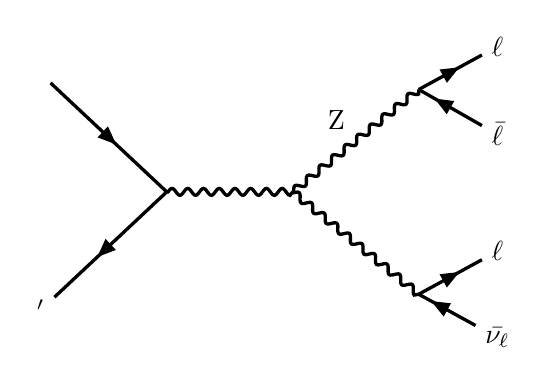
\begin{tikzpicture} % WZ at LO (s-channel)
  \begin{feynman}
   \vertex (q1) {\(\boldsymbol{\Pq}\)};
   \vertex [below= 3cm of q1] (q2) {\(\boldsymbol{\Paq'}\)};
   \vertex [right= 1.6cm of q1] (a1);
   \vertex [below= 1.5cm of a1] (a2);
   \vertex [right= 1.6cm of a2] (b1);
   \vertex [right= 1.6cm of b1] (c1);
   \vertex [above= 1.3cm of c1] (c2);
   \vertex [below= 1.3cm of c1] (c3);
   \vertex [right= 1cm of c2] (d1);
   \vertex [right= 1cm of c3] (d2);
   \vertex [above= 0.3cm of d1] (f1) {\(\boldsymbol{\ell}\)};
   \vertex [below= 0.3cm of d1] (f2) {\(\boldsymbol{\bar{\ell}}\)};
   \vertex [above= 0.3cm of d2] (f3) {\(\boldsymbol{\ell}\)};
   \vertex [below= 0.3cm of d2] (f4) {\(\boldsymbol{\bar{\nu_\ell}}\)};
   
   \diagram* {
    (q1) -- [fermion, very thick] (a2),
    (q2) -- [anti fermion, very thick] (a2),
    (a2) -- [boson, very thick, edge label'=\(\boldsymbol{\PWm}\)] (b1),
    (b1) -- [boson, very thick, edge label=\(\boldsymbol{\Z}\)] (c2),
    (b1) -- [boson, very thick, edge label=\(\boldsymbol{\PWm}\)] (c3),
    (c2) -- [fermion, very thick] (f1),
    (c2) -- [anti fermion, very thick] (f2),
    (c3) -- [fermion, very thick] (f3),
    (c3) -- [anti fermion, very thick] (f4),
   };
  \end{feynman}
 \end{tikzpicture} \hspace{1cm}
 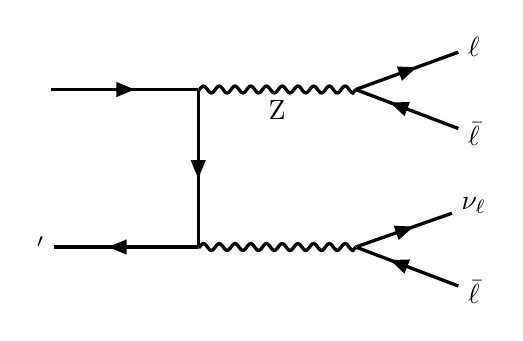
\begin{tikzpicture} % WZ at LO (t-channel)
  \begin{feynman}
   \vertex (q1) {\(\boldsymbol{\Pq}\)};
   \vertex [below= 2cm of q1] (q2) {\(\boldsymbol{\Paq'}\)};
   \vertex [right= 2cm of q1] (a);
   \vertex [right= 2cm of q2] (b);
   \vertex [right= 2cm of a] (c);
   \vertex [right= 2cm of b] (d);
   \vertex [right= 1.5cm of c] (e);
   \vertex [right= 1.5cm of d] (f);
   \vertex [above= 0.3cm of e] (f1) {\(\boldsymbol{\ell}\)};
   \vertex [below= 0.3cm of e] (f2) {\(\boldsymbol{\bar{\ell}}\)};
   \vertex [above= 0.3cm of f] (f3) {\(\boldsymbol{\nu_\ell}\)};
   \vertex [below= 0.3cm of f] (f4) {\(\boldsymbol{\bar{\ell}}\)};
   
   \diagram* {
    (q1) -- [fermion, very thick] (a),
    (q2) -- [anti fermion, very thick] (b),
    (a) -- [fermion, very thick] (b),
    (a) -- [boson, very thick, edge label'=\(\boldsymbol{\Z}\)] (c),
    (b) -- [boson, very thick, edge label'=\(\boldsymbol{\PWp}\)] (d),
    (c) -- [fermion, very thick] (f1),
    (c) -- [anti fermion, very thick] (f2),
    (d) -- [fermion, very thick] (f3),
    (d) -- [anti fermion, very thick] (f4),
   };
  \end{feynman}
 \end{tikzpicture}  
 \caption{Leading order WZ production mechanisms in the $s$-channel and the $t$-channel.} \label{fig:WZLO}
\end{figure}

\begin{figure} % WZ NLO EW
 \centering
 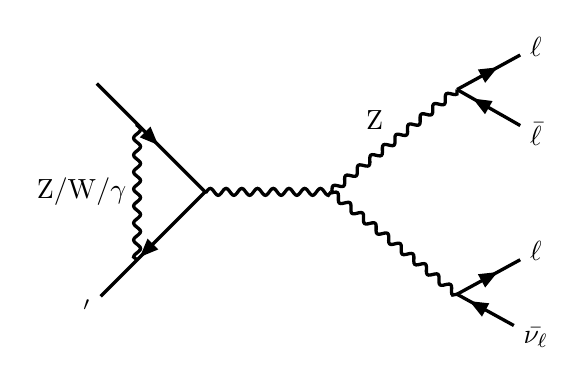
\begin{tikzpicture} % WZ at NLO EW (s-channel) internal loop
  \begin{feynman}
   \vertex (q1) {\(\boldsymbol{\Pq}\)};
   \vertex [below= 3cm of q1] (q2) {\(\boldsymbol{\Paq'}\)};
   \vertex [right= 1.5cm of q1] (a1);
   \vertex [below= 1.5cm of a1] (a2);
   \vertex [right= 1.6cm of a2] (b1);
   \vertex [right= 1.6cm of b1] (c1);
   \vertex [above= 1.3cm of c1] (c2);
   \vertex [below= 1.3cm of c1] (c3);
   \vertex [right= 1cm of c2] (d1);
   \vertex [right= 1cm of c3] (d2);
   \vertex [above= 0.3cm of d1] (f1) {\(\boldsymbol{\ell}\)};
   \vertex [below= 0.3cm of d1] (f2) {\(\boldsymbol{\bar{\ell}}\)};
   \vertex [above= 0.3cm of d2] (f3) {\(\boldsymbol{\ell}\)};
   \vertex [below= 0.3cm of d2] (f4) {\(\boldsymbol{\bar{\nu_\ell}}\)};
   \vertex [below right= 0.9cm of q1] (V1);
   \vertex [above right= 0.9cm of q2] (V2);
   
   \diagram* {
    (q1) -- [fermion, very thick] (a2),
    (q2) -- [anti fermion, very thick] (a2),
    (a2) -- [boson, very thick, edge label'=\(\boldsymbol{\PWm}\)] (b1),
    (b1) -- [boson, very thick, edge label=\(\boldsymbol{\Z}\)] (c2),
    (b1) -- [boson, very thick, edge label=\(\boldsymbol{\PWm}\)] (c3),
    (c2) -- [fermion, very thick] (f1),
    (c2) -- [anti fermion, very thick] (f2),
    (c3) -- [fermion, very thick] (f3),
    (c3) -- [anti fermion, very thick] (f4),
    (V1) -- [boson, very thick, edge label'=\(\boldsymbol{\Z/\W/\gamma}\)] (V2),
   };
  \end{feynman}
 \end{tikzpicture} \hspace{1cm}
 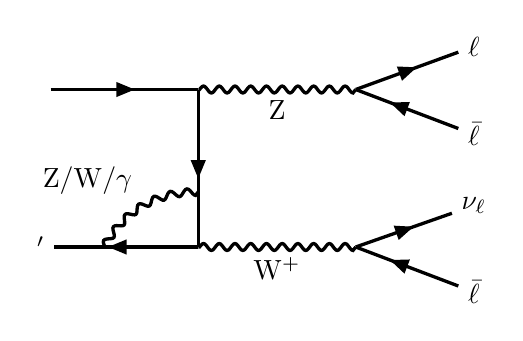
\begin{tikzpicture} % WZ at NLO (t-channel) internal loop
  \begin{feynman}
   \vertex (q1) {\(\boldsymbol{\Pq}\)};
   \vertex [below= 2cm of q1] (q2) {\(\boldsymbol{\Paq'}\)};
   \vertex [right= 2cm of q1] (a);
   \vertex [right= 2cm of q2] (b);
   \vertex [right= 2cm of a] (c);
   \vertex [right= 2cm of b] (d);
   \vertex [right= 1.5cm of c] (e);
   \vertex [right= 1.5cm of d] (f);
   \vertex [above= 0.3cm of e] (f1) {\(\boldsymbol{\ell}\)};
   \vertex [below= 0.3cm of e] (f2) {\(\boldsymbol{\bar{\ell}}\)};
   \vertex [above= 0.3cm of f] (f3) {\(\boldsymbol{\nu_\ell}\)};
   \vertex [below= 0.3cm of f] (f4) {\(\boldsymbol{\bar{\ell}}\)};
   \vertex [right= 0.8cm of q2] (V1);
   \vertex [above= 0.7cm of b] (V2);
   
   \diagram* {
    (q1) -- [fermion, very thick] (a),
    (q2) -- [anti fermion, very thick] (b),
    (a) -- [fermion, very thick] (b),
    (a) -- [boson, very thick, edge label'=\(\boldsymbol{\Z}\)] (c),
    (b) -- [boson, very thick, edge label'=\(\boldsymbol{\W^+}\)] (d),
    (c) -- [fermion, very thick] (f1),
    (c) -- [anti fermion, very thick] (f2),
    (d) -- [fermion, very thick] (f3),
    (d) -- [anti fermion, very thick] (f4),
    (V1) -- [boson, very thick, bend left, edge label=\(\boldsymbol{\Z/\W/\gamma}\)] (V2),
   };
  \end{feynman}
 \end{tikzpicture} \vspace{1cm}

 \begin{tikzpicture} % WZ at NLO EW (s-channel) y-induced
  \begin{feynman}
   \vertex (y1) {\(\boldsymbol{\gamma}\)};
   \vertex [below= 3cm of y1] (q2) {\(\boldsymbol{\Pq}\)};
   \vertex [right= 1.5cm of q1] (a1);
   \vertex [below= 1.5cm of a1] (a2);
   \vertex [right= 1.6cm of a2] (b1);
   \vertex [right= 1.6cm of b1] (c1);
   \vertex [above= 1.3cm of c1] (c2);
   \vertex [below= 1.3cm of c1] (c3);
   \vertex [right= 1cm of c2] (d1);
   \vertex [right= 1cm of c3] (d2);
   \vertex [above= 0.3cm of d1] (f1) {\(\boldsymbol{\ell}\)};
   \vertex [below= 0.3cm of d1] (f2) {\(\boldsymbol{\bar{\ell}}\)};
   \vertex [above= 0.3cm of d2] (f3) {\(\boldsymbol{\ell}\)};
   \vertex [below= 0.3cm of d2] (f4) {\(\boldsymbol{\bar{\nu_\ell}}\)};
   \vertex [below right= 1.2cm of y1] (y2);
   \vertex [right= 1cm of y2] (fsrq1);
   \vertex [above= 0.6cm of fsrq1] (fsrq2) {\(\boldsymbol{\Pq'}\)};
   
   \diagram* {
    (y1) -- [boson, very thick] (y2),
    (y2) -- [anti fermion, very thick] (a2),
    (q2) -- [fermion, very thick] (a2),
    (a2) -- [boson, very thick, edge label'=\(\boldsymbol{\PWm}\)] (b1),
    (b1) -- [boson, very thick, edge label=\(\boldsymbol{\Z}\)] (c2),
    (b1) -- [boson, very thick, edge label=\(\boldsymbol{\PWm}\)] (c3),
    (c2) -- [fermion, very thick] (f1),
    (c2) -- [anti fermion, very thick] (f2),
    (c3) -- [fermion, very thick] (f3),
    (c3) -- [anti fermion, very thick] (f4),
    (y2) -- [fermion, very thick] (fsrq2),
   };
  \end{feynman}
 \end{tikzpicture} \hspace{1cm}
 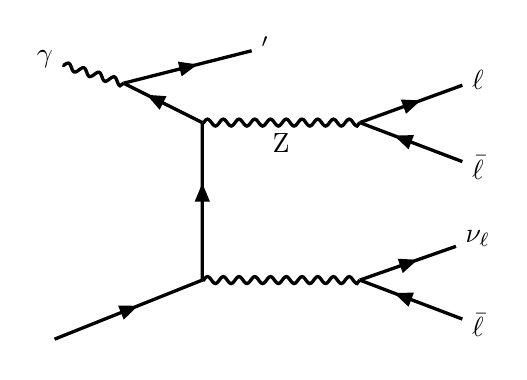
\begin{tikzpicture} % WZ at NLO EW (t-channel) y-induced
  \begin{feynman}
   \vertex (y1) {\(\boldsymbol{\gamma}\)};
   \vertex [right= 1cm of y1] (y2);
   \vertex [below= 0.3cm of y2] (y3);
   \vertex [right= 1.8cm of y3] (fsrq1);
   \vertex [above= 0.2cm of fsrq1] (fsrq2) {\(\boldsymbol{\Pq'}\)};
   \vertex [below= 3.6cm of y1] (q2) {\(\boldsymbol{\Pq}\)};
   \vertex [right= 1cm of y3] (a1);
   \vertex [below= 0.5cm of a1] (a2);
   \vertex [right= 2cm of q2] (a3);
   \vertex [above= 0.8cm of a3] (a4);
   \vertex [right= 2cm of a2] (c);
   \vertex [right= 2cm of a4] (d);
   \vertex [right= 1.5cm of c] (e);
   \vertex [right= 1.5cm of d] (f);
   \vertex [above= 0.3cm of e] (f1) {\(\boldsymbol{\ell}\)};
   \vertex [below= 0.3cm of e] (f2) {\(\boldsymbol{\bar{\ell}}\)};
   \vertex [above= 0.3cm of f] (f3) {\(\boldsymbol{\nu_\ell}\)};
   \vertex [below= 0.3cm of f] (f4) {\(\boldsymbol{\bar{\ell}}\)};
   
   \diagram* {
    (y1) -- [boson, very thick] (y3),
    (y3) -- [anti fermion, very thick] (a2),
    (q2) -- [fermion, very thick] (a4),
    (a2) -- [anti fermion, very thick] (a4),
    (a2) -- [boson, very thick, edge label'=\(\boldsymbol{\Z}\)] (c),
    (a4) -- [boson, very thick, edge label'=\(\boldsymbol{\PWp}\)] (d),
    (c) -- [fermion, very thick] (f1),
    (c) -- [anti fermion, very thick] (f2),
    (d) -- [fermion, very thick] (f3),
    (d) -- [anti fermion, very thick] (f4),
    (y3) -- [fermion, very thick] (fsrq2),
   };
  \end{feynman}
 \end{tikzpicture}  
 

 \caption{WZ production at NLO in EW by internal loop processes (upper row) and photon-quark induced processes (lower row).} \label{fig:ZZto4l}
\end{figure}

\begin{figure} % BSM models
 \centering
 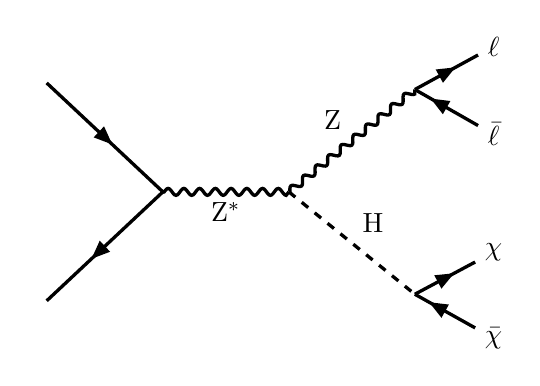
\begin{tikzpicture} % ZH(inv)
  \begin{feynman}
   \vertex (q1) {\(\boldsymbol{\Pq}\)};
   \vertex [below= 3cm of q1] (q2) {\(\boldsymbol{\Paq}\)};
   \vertex [right= 1.6cm of q1] (a1);
   \vertex [below= 1.5cm of a1] (a2);
   \vertex [right= 1.6cm of a2] (b1);
   \vertex [right= 1.6cm of b1] (c1);
   \vertex [above= 1.3cm of c1] (c2);
   \vertex [below= 1.3cm of c1] (c3);
   \vertex [right= 1cm of c2] (d1);
   \vertex [right= 1cm of c3] (d2);
   \vertex [above= 0.3cm of d1] (f1) {\(\boldsymbol{\ell}\)};
   \vertex [below= 0.3cm of d1] (f2) {\(\boldsymbol{\bar{\ell}}\)};
   \vertex [above= 0.3cm of d2] (f3) {\(\boldsymbol{\chi}\)};
   \vertex [below= 0.3cm of d2] (f4) {\(\boldsymbol{\bar{\chi}}\)};
   
   \diagram* {
    (q1) -- [fermion, very thick] (a2),
    (q2) -- [anti fermion, very thick] (a2),
    (a2) -- [boson, very thick, edge label'=\(\boldsymbol{\Z^*}\)] (b1),
    (b1) -- [boson, very thick, edge label=\(\boldsymbol{\Z}\)] (c2),
    (b1) -- [scalar, very thick, edge label=\(\boldsymbol{\Hi}\)] (c3),
    (c2) -- [fermion, very thick] (f1),
    (c2) -- [anti fermion, very thick] (f2),
    (c3) -- [fermion, very thick] (f3),
    (c3) -- [anti fermion, very thick] (f4),
   };
  \end{feynman}
 \end{tikzpicture} \hspace{1cm}
 \begin{tikzpicture} % Simplified model spin-0 mediator
  \begin{feynman}
   \vertex (g1) {\(\boldsymbol{}\)};
   \vertex [below= 3.6cm of g1] (g2) {\(\boldsymbol{}\)};
   \vertex [right= 1.4cm of g1] (a1);
   \vertex [right= 1.4cm of g2] (a2);
   \vertex [below= 0.8cm of a1] (a3);
   \vertex [above= 0.8cm of a2] (a4);
   \vertex [right= 1.4cm of a3] (b1);
   \vertex [right= 1.4cm of a4] (b2);
   \vertex [right= 1.4cm of b1] (c1);
   \vertex [right= 1.4cm of b2] (c2);
   \vertex [right= 1cm of c1] (d1);
   \vertex [right= 1cm of c2] (d2);
   \vertex [above= 0.3cm of d1] (f1) {\(\boldsymbol{\ell}\)};
   \vertex [below= 0.3cm of d1] (f2) {\(\boldsymbol{\bar{\ell}}\)};
   \vertex [above= 0.3cm of d2] (f3) {\(\boldsymbol{\chi}\)};
   \vertex [below= 0.3cm of d2] (f4) {\(\boldsymbol{\bar{\chi}}\)};
   \vertex [below = 0.2cm of b2] (dm1) {\(\boldsymbol{g_\Pq}\)};
   \vertex [below = 0.2cm of c2] (dm2) {\(\boldsymbol{g_\mathrm{DM}}\)};
   
   \diagram* {
    (g1) -- [gluon, very thick] (a3),
    (g2) -- [gluon, very thick] (a4),
    (a3) -- [fermion, very thick, edge label'=\(\boldsymbol{\bar{\Top}}\)] (a4) -- [fermion, very thick, edge label=\(\boldsymbol{\Top}\)] (b2) -- [fermion, very thick, edge label=\(\boldsymbol{\bar{\Top}}\)] (b1) -- [fermion, very thick, edge label'=\(\boldsymbol{\Top}\)] (a3),
    (b1) -- [boson, very thick, edge label=\(\boldsymbol{\Z}\)] (c1),
    (b2) -- [scalar, very thick, edge label=\(\boldsymbol{\phi}\)] (c2),
    (c1) -- [fermion, very thick] (f1),
    (c1) -- [anti fermion, very thick] (f2),
    (c2) -- [fermion, very thick] (f3),
    (c2) -- [anti fermion, very thick] (f4),
   };
  \draw[fill=blue,line width=0pt] (b2) circle(1.5mm);
  \draw[fill=violet,line width=0pt] (c2) circle(1.5mm);
  \end{feynman}
 \end{tikzpicture} \vspace{1cm}
 
 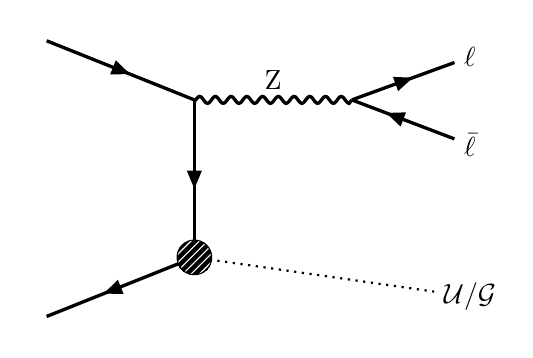
\begin{tikzpicture} % Simplified model spin-1 mediator
  \begin{feynman}
   \vertex (q1) {\(\boldsymbol{\Pq}\)};
   \vertex [below= 3.6cm of q1] (q2) {\(\boldsymbol{\Paq}\)};
   \vertex [right= 2cm of q1] (a1);
   \vertex [right= 2cm of q2] (a2);
   \vertex [below= 0.8cm of a1] (a3);
   \vertex [above= 0.8cm of a2] (a4);
   \vertex [right= 2cm of a3] (b1);
   \vertex [right= 2cm of a4] (b2);
   \vertex [right= 1.5cm of b1] (c1);
   \vertex [right= 1.5cm of b2] (c2);
   \vertex [above= 0.3cm of c1] (f1) {\(\boldsymbol{\ell}\)};
   \vertex [below= 0.3cm of c1] (f2) {\(\boldsymbol{\bar{\ell}}\)};
   \vertex [below= 0.2cm of c2] (U) {\(\boldsymbol{\mathcal{U}/\mathcal{G}}\)};
   
   \diagram* {
    (q1) -- [fermion, very thick] (a3),
    (a3) -- [fermion, very thick] (a4),
    (q2) -- [anti fermion, very thick] (a4),
    (a3) -- [boson, very thick, edge label=\(\boldsymbol{\Z}\)] (b1),
    (a4) -- [ghost, very thick] (U),
    (b1) -- [fermion, very thick] (f1),
    (b1) -- [anti fermion, very thick] (f2),
   };
  \draw[fill=black,line width=0pt] (a4) circle(2.2mm);
  \draw[pattern=north east lines, pattern color=white] (a4) circle(2.2mm);
  \end{feynman}
 \end{tikzpicture} \hspace{1cm}  
 \begin{tikzpicture} % ADD/unparticles
  \begin{feynman}
   \vertex (q1) {\(\boldsymbol{\Pq}\)};
   \vertex [below= 3.6cm of q1] (q2) {\(\boldsymbol{\Paq}\)};
   \vertex [right= 2cm of q1] (a1);
   \vertex [right= 2cm of q2] (a2);
   \vertex [below= 0.8cm of a1] (a3);
   \vertex [above= 0.8cm of a2] (a4);
   \vertex [right= 2cm of a3] (b1);
   \vertex [right= 2cm of a4] (b2);
   \vertex [right= 1.5cm of b1] (c1);
   \vertex [right= 1.5cm of b2] (c2);
   \vertex [above= 0.3cm of c1] (f1) {\(\boldsymbol{\ell}\)};
   \vertex [below= 0.3cm of c1] (f2) {\(\boldsymbol{\bar{\ell}}\)};
   \vertex [above= 0.3cm of c2] (f3) {\(\boldsymbol{\chi}\)};
   \vertex [below= 0.3cm of c2] (f4) {\(\boldsymbol{\bar{\chi}}\)};
   \vertex [below = 0.2cm of a4] (dm1) {\(\boldsymbol{g_\Pq}\)};
   \vertex [below = 0.2cm of b2] (dm2) {\(\boldsymbol{g_\mathrm{DM}}\)};
   
   \diagram* {
    (q1) -- [fermion, very thick] (a3),
    (a3) -- [fermion, very thick] (a4),
    (q2) -- [anti fermion, very thick] (a4),
    (a3) -- [boson, very thick, edge label=\(\boldsymbol{\Z}\)] (b1),
    (a4) -- [boson, very thick, edge label=\(\boldsymbol{\mathcal{A}}\)] (b2),
    (b1) -- [fermion, very thick] (f1),
    (b1) -- [anti fermion, very thick] (f2),
    (b2) -- [fermion, very thick] (f3),
    (b2) -- [anti fermion, very thick] (f4),
   };
  \draw[fill=blue,line width=0pt] (a4) circle(1.5mm);
  \draw[fill=violet,line width=0pt] (b2) circle(1.5mm);
  \end{feynman}
 \end{tikzpicture}
 \caption{Some diagrams beyond the Standard Model in which are produced two charged leptons and missing energy. Clockwise from upper left: associated production of an invisible Higgs boson; gluon-induced production of a Z boson and a massive spin-0 dark matter mediator via top-quark loop; production of a Z boson and a massive spin-1 dark matter mediator; production of a Z boson in association with gravitons (ADD model) or unparticles.} \label{fig:BSMdiagrams}
 \end{figure}
\end{document}
